\newcommand{\psd}[1]{{\small\sffamily{\color{blue!60}#1}}}

To showcase the usage of Linear elasticity, we shall discuss here an
example of a 2D bar, which bends under its own load. The bar
\(5\times1\) m\(^2\) in area is made up of material with
\(\rho=8\times 10^3\), \(E=200\times 10^9\), and \(\nu=0.3\).

\begin{figure}[h!]
\centering
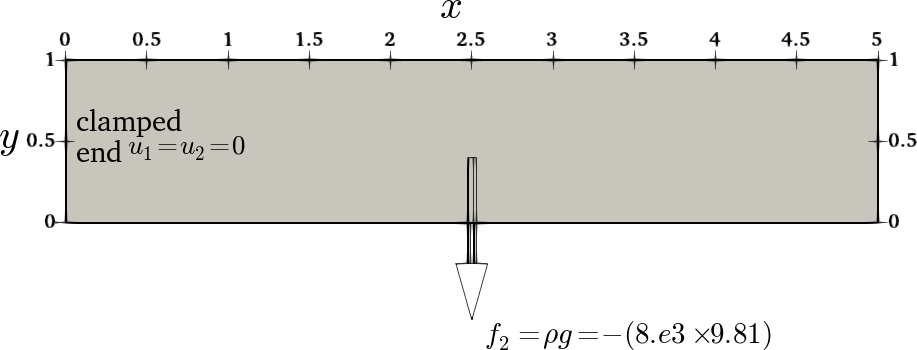
\includegraphics[width=0.5\textwidth]{./Images/le-2d-bar.png}
\caption{The 2D clamped bar problem. \label{2dbar-le-full}}
\end{figure}

\subsection{Step 1: Preprocessing}

First step in a PSD simulation is PSD preprocessing, at this step you
tell PSD what kind of physics, boundary conditions, approximations,
mesh, etc are you expecting to solve.

In the terminal \psd{cd} to the folder
\psd{/home/PSD-tutorials/linear-elasticity}
\footnote{Note that one can perform these simulation in any folder provided that PSD has been properly installed. We use \psd{/home/PSD-tutorials/linear-elasticity} for simplicity, once the user is proficient a simulation can be launch elsewhere.}.
Launch \psd{PSD\_PreProcess} from the terminal, to do so run the
following command.

\begin{lstlisting}[style=BashInputStyle]
PSD_PreProcess -problem linear_elasticity -dimension 2 -bodyforceconditions 1 \
-dirichletconditions 1 -postprocess u
\end{lstlisting}

After the \psd{PSD\_PreProcess} runs successfully you should see many
\psd{.edp} files in your current folder.

\textbf{What do the arguments mean ?}

\begin{itemize}
\item \psd{-problem linear\_elasticity} means that we are solving linear elasticity problem;
\item \psd{-dimension 2} means it is a 2D simulation;
\item \psd{-bodyforceconditions 1} with applied body force acting on the domain;
\item \psd{-dirichletconditions 1} says we have one Dirichlet border;
\item \psd{-postprocess u} means we would like to have ParaView post processing files.
\end{itemize}

At this stage the input properties \(E,\nu\) can be mentioned in
\psd{ControlParameters.edp}, use \psd{E = 200.e9}, and \psd{nu = 0.3;}.
The volumetric body force condition is mentioned in the same file via
variable \psd{Fbc0Fy -78480.0}, i.e (\(\rho*g=8.e3*(-9.81)=-78480.0\)).
One can also provide the mesh to be used in \psd{ControlParameters.edp},
via \psd{ThName = "../Meshes/2D/bar.msh"}
(\textit{note that mesh can also be provided in the next step}) .In
addition variable \psd{Fbc0On 1} has to be provided in order to indicate
the volume (region) for which the body force is acting, here \psd{1} is
the integer volume tag of the mesh. Dirichlet boundary conditions are
also provided in \psd{ControlParameters.edp}. To provide the clamped
boundary condition the variables \psd{Dbc0On 2}, \psd{Dbc0Ux 0.}, and
\psd{Dbc0Uy 0.} are used, which means for Dirichlet border \psd{2}
(\psd{Dbc0On 2}) where \psd{2} is the clamped border label of the mesh
Dirichlet constrain is applied and \psd{Dbc0Ux 0.}, \psd{Dbc0Uy 0} i.e.,
the clamped end condition (\(u_x=u_y=0\)).

\subsection{Step 2: Solving}

As PSD is a parallel solver, let us use 4 cores to solve the 2D bar
case. To do so enter the following command:

\begin{lstlisting}[style=BashInputStyle]
PSD_Solve -np 4 Main.edp -mesh ./../Meshes/2D/bar.msh -v 0
\end{lstlisting}

Here \psd{-np 4} denote the argument used to enter the number of
parallel processes (MPI processes) used while solving.
\psd{-mesh ./../Meshes/2D/bar.msh} is used to provide the mesh file to
the solver. \psd{-v 0} denotes the verbosity level on screen.
\psd{PSD\_Solve} is a wrapper around \psd{FreeFem++} or
\psd{FreeFem++-mpi}. Note that if your problem is large use more cores.
PSD has been tested upto 13,000 parallel processes and problem sizes
with billions of unknowns, surely you will now need that many for the 2D
bar problem.

\subsection{Step 3: Postprocessing}

PSD allows postprocessing of results in ParaView. After the step 2
mentioned above finishes. Launch ParaView and have a look at the
\psd{.pvd} file in the \psd{VTUs...} folder. Using ParaView for
postprocessing the results that are provided in the \psd{VTUs...}
folder, results such as those shown in
figure\textasciitilde{}\ref{bar-le-full} can be extracted.

\begin{figure}[h!]
\centering
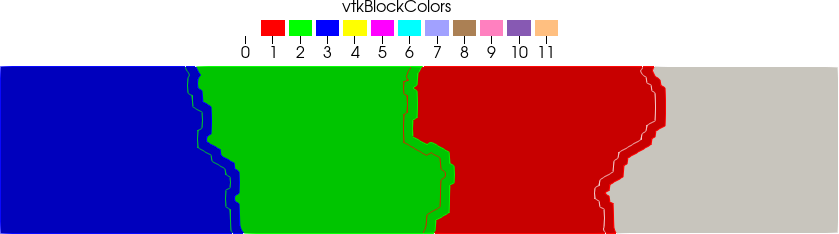
\includegraphics[width=0.4\textwidth]{./Images/le-2d-bar-partioned.png}\\
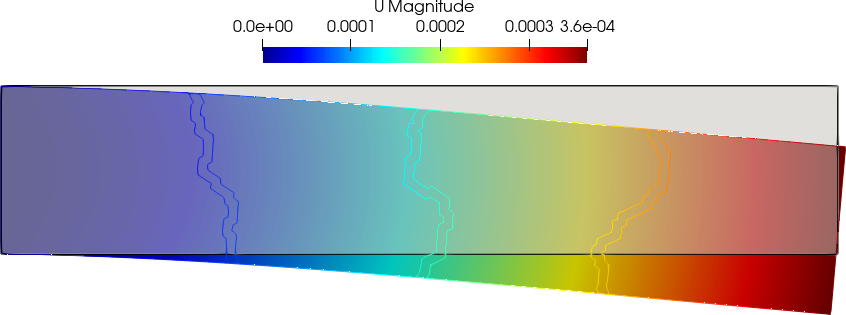
\includegraphics[width=0.4\textwidth]{./Images/le-2d-bar-results.png}
\caption{The 2D clamped bar problem: partitioned mesh and displacement field visualization in ParaView. \label{bar-le-full}}
\end{figure}

You are all done with your 2D linear-elasticty simulation.

\subsection{2D bar is ok, but what about 3D ?}

3D follows the same logic as 2D, in the preprocessing step

\begin{lstlisting}[style=BashInputStyle]
PSD_PreProcess -problem linear_elasticity -dimension 3 -bodyforceconditions 1 \
-dirichletconditions 1 -postprocess u
\end{lstlisting}

note that all what has changed \psd{-dimension 3} instead of
\psd{-dimension 2}

Solving step remains exactly the same with \psd{-mesh} flag now pointing
towards the \psd{3D} mesh.

\begin{lstlisting}[style=BashInputStyle]
PSD_Solve -np 4 Main.edp -mesh ./../Meshes/3D/bar.msh -v 0
\end{lstlisting}

\begin{figure}[h!]
\centering
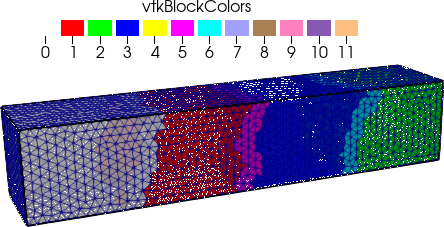
\includegraphics[width=0.4\textwidth]{./Images/le-3d-bar-clamped-ends.png}\\
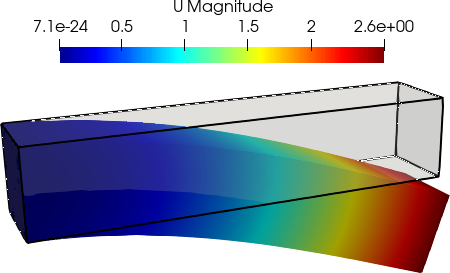
\includegraphics[width=0.4\textwidth]{./Images/le-3d-bar-clamped-pulled-partioned.png}
\caption{The 3D clamped bar problem: partitioned mesh and displacement field visualization in ParaView. \label{3dbar-le-full}}
\end{figure}

Using ParaView for postprocessing the results that are provided in the
\psd{VTUs...} folder, results such as those shown in
figure\textasciitilde{}\ref{3dbar-le-full} can be extracted.

\subsection{Solving using a sequential solver (non parallel)}

To the same problems above Add \sh{-sequential} flag to
\sh{PSD\_PreProcess} for sequential solver, but remember to use
\sh{PSD\_Solve\_Seq} instead of \sh{PSD\_Solve}. So the work flow for
the 2D problem would be:

\begin{lstlisting}[style=BashInputStyle]
PSD_PreProcess -problem linear_elasticity -dimension 2 -bodyforceconditions 1 \
-dirichletconditions 1 -postprocess u -sequential
\end{lstlisting}

We solve the problem using the given mesh file \sh{bar.msh}.

\begin{lstlisting}[style=BashInputStyle]
PSD_Solve_Seq Main.edp -mesh ./../Meshes/2D/bar.msh -v 0
\end{lstlisting}

Similarly try out the 3D problem as well.

\subsection{Comparing CPU time}

PSD provides mean to time log your solver via \sh{-timelog} flag. What
this will do when you run your solver, on the terminal you will have
information printed on what is the amount of time taken by each step of
your solver. Warning, this will make your solver slower, as this action
involves `MPI\_Barrier' routines for correctly timing operation.

An example work flow of 2D solver with timelogging:

\begin{lstlisting}[style=BashInputStyle]
PSD_PreProcess -problem linear_elasticity -dimension 2 -bodyforceconditions 1 \
-dirichletconditions 1 -postprocess u -timelog
\end{lstlisting}

We solve the problem using four MPI processes, with the given mesh file
\sh{bar.msh}.

\begin{lstlisting}[style=BashInputStyle]
PSD_Solve -np 4 Main.edp -mesh ./../Meshes/2D/bar.msh -v 0
\end{lstlisting}

\begin{figure}[h!]
\centering
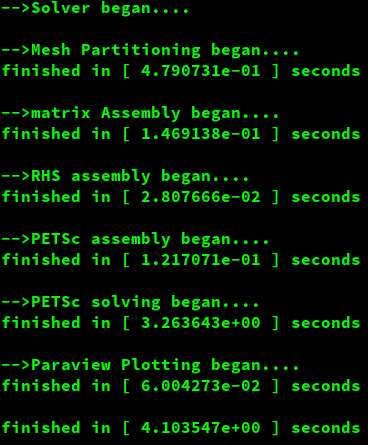
\includegraphics[width=0.4\textwidth]{./Images/le-time-par.png}
\caption{Time logging output produced for parallel run on 4 processes.\label{time-par-le}}
\end{figure}

The figure\textasciitilde{}\ref{time-par-le} shows the time logging
output produced for parallel run on 4 processes using \sh{-timelog}
flag. Take note of timings produced for different operations of the
solver.

You are encouraged to use more complex meshes for this same problem, but
do not forget to update the \psd{ControlParameters.edp} file.

\subsection{Advance exercise  1}

There is a solver run level flag for mesh refinement
\footnote{Mesh refinement is performed after partitioning.}. This flag
is called \psd{-split [int]} which splits the triangles (resp.
tetrahedrons) of your mesh into four smaller triangles (resp.
tetrahedrons). As such \psd{-split 2} will produce a mesh with 4 times
the elements of the input mesh. Similarly, \psd{-split n} where \(n\) is
a positive integer produces \(2^n\) times more elements than the input
mesh. You are encouraged to use this \psd{-split} flag to produce
refined meshes and check, mesh convergence of a problem, computational
time, etc. Use of parallel computing is recommended. You could try it
out with \psd{PSD\_Solve} or \psd{PSD\_Solve\_Seq}, for example:

\begin{lstlisting}[style=BashInputStyle]
PSD_Solve -np 4 Main.edp -mesh ./../Meshes/2D/bar.msh -v 0 -split 2
\end{lstlisting}

for splitting each triangle of the mesh \psd{bar.msh} into 4.

\subsection{Advance exercise  2}

There is a preprocess level flag \psd{-debug}, which as the name
suggests should be used for debug proposes by developers. However, this
flag will activate OpenGL live visualization of the problems
displacement field. You are encouraged to try it out

\begin{lstlisting}[style=BashInputStyle]
PSD_PreProcess -problem linear_elasticity -dimension 2 -bodyforceconditions 1 \
-dirichletconditions 1 -postprocess u -timelog -debug
\end{lstlisting}

Then to run the problem we need additional \psd{-wg} flag

\begin{lstlisting}[style=BashInputStyle]
PSD_Solve -np 4 Main.edp -mesh ./../Meshes/2D/bar.msh -v 0 -wg
\end{lstlisting}

\subsection{Exercise  3}

One interesting way of solving a linear Elasticity problem is to solve
it via a pseudo nonlinear model. There is a preprocess level flag
\psd{-model pseudo\_nonlinear}, which introduces pseudo nonlinearity
into the finite element variational formulation of linear elasticity.
You are encouraged to use this flag and see how the solver performs.
Indeed, now you should see some nonlinear iterations (1 or 2) are taken
for convergence.

\begin{lstlisting}[style=BashInputStyle]
PSD_PreProcess -problem linear_elasticity -dimension 2 -bodyforceconditions 1 \
-dirichletconditions 1 -postprocess u -timelog -model pseudo_nonlinear
\end{lstlisting}

Then to run the problem

\begin{lstlisting}[style=BashInputStyle]
PSD_Solve -np 4 Main.edp -mesh ./../Meshes/2D/bar.msh -v 0
\end{lstlisting}

To understand what the flag does, try to find out the difference between
the files created by \psd{PSD\_PreProcess} when used with and without
\psd{-model pseudo\_nonlinear} flag. Especially, compare
\psd{LinearFormBuilderAndSolver.edp} and
\psd{VariationalFormulations.edp} files produced by
\psd{PSD\_PreProcess} step. You will see Newton--Raphsons iterations are
performed for solving the linear problem. However, the nonlinear
iterations loop converges very rapidly (in 1 iteration) due to linear
nature of the problem. \textbf{Note:} This flag is exclusive for
parallel solver.

\subsection{Advance exercise 4}

There is a preprocess level flag \psd{-withmaterialtensor}, which
introduces the full material tensor into the finite element variational
formulation. You are encouraged to use this flag and see how the solver
performs.

\begin{lstlisting}[style=BashInputStyle]
PSD_PreProcess -problem linear_elasticity -dimension 2 -bodyforceconditions 1 \
-dirichletconditions 1 -postprocess u -timelog -withmaterialtensor
\end{lstlisting}

Then to run the problem

\begin{lstlisting}[style=BashInputStyle]
PSD_Solve -np 4 Main.edp -mesh ./../Meshes/2D/bar.msh -v 0
\end{lstlisting}

To understand what the flag does, try to find out the difference between
the files created by \psd{PSD\_PreProcess} when used with and without
\psd{-withmaterialtensor} flag. Especially, compare
\psd{FemParameters.edp}, \psd{MeshAndFeSpace} and
\psd{VariationalFormulations.edp} files produced by
\psd{PSD\_PreProcess} step.
